\section{Linked Data}

Het semantisch web gaat echter niet enkel over het plaatsen van data op het web. Het belangrijkste aspect van het semantisch web is het maken van links, zodat zowel personen als machines het web van data kunnen doorkruisen. Het belangrijke van gelinkte data is hetvolgende: wanneer je data hebt, kan je er andere gerelateerde data mee vinden. Bij gelinkte data worden deze links beschreven aan de hand van RDF. Hierbij worden URI's gebruiks voor het identificeren van objecten. Om data te interconnecteren zijn er vier regels, met als doen dat de informatie in de toekomst op onvoorspelbare manieren herbruikt zou kunnen worden. Daarnaast is het belangrijk dat de data open en toegankelijk is om herbruikt te worden \cite{berners2006linkeddata}. 

\subsection{Regels}
De eerste regel is om dingen te identificeren met URI's. Dit is nodig om te kunnen spreken over een semantisch web \cite{berners2006linkeddata}. 

De tweede regel is het gebruiken van HTTP URI's. Deze tweede regel is nodig zodat andere gebruikers de namen zouden kunnen opzoeken \cite{berners2006linkeddata}. 

De derde regel is dat bijhorende informatie gevonden moet kunnen worden wanneer een URI gevolgd wordt. Dit is in het basis formaat van RDF en XML. Deze kan ook doorzocht worden aan de hand van SPARQL (verder besproken in \sectionref{sec:sparql}), dit is een query service voor gelinkte data in RDF formaat \cite{berners2006linkeddata}. 

De vierde regel is het voorzien van links naar andere locaties die gelijkaardige data bevat, zodat dit opgezocht kan worden. Deze laatste regel is belangrijk om de informatie op het web te connecteren \cite{berners2006linkeddata}.

\subsection{Vijf sterren model}
Het vijf sterren model is een manier om informatie in te delen in hoeverre ze open is. Meer sterren betekent dat de informatie meer open is. Tim Berners-Lee stelde dit model voor als schema voor gelinkte open data. Gelinkte open data is namelijk een essentiëel onderdeel van het semantisch web.

Eén ster stelt hetvolgende: ``\textit{Available on the web but with an open licence, to be Open Data}''. Dit betekent dat gebruikers informatie kunnen ophalen, gebruiken en delen met iedereen. Het gaat hier echter louter over het delen van informatie, het maakt dus niet uit in welk formaat dit komt \cite{berners2006linkeddata}. 

Twee sterren stelt dan weer: ``\textit{Available as machine-readable structured data}''. Om twee sterren te krijgen is het belangrijk dat de informatie een bepaalde structuur heeft, zodat machines deze informatie kunnen verwerken. Dit kan bijvoorbeeld zijn in de vorm van een excel spreadsheet. Dit soort informatie is echter nog steeds vrij gesloten aangezien de gebruikers afhankelijk zijn van bepaalde software om toegang te krijgen tot de informatie \cite{berners2006linkeddata}.

Drie sterren betekent: ``\textit{The same as 2 stars, plus non-proprietary format}''. Het verschil om van twee sterren naar drie sterren te stijgen is het vermijden van de nood aan specifieke software om de informatie te bemachtigen. Dit kan bijvoorbeeld door de informatie op te slaan in CSV formaat \cite{berners2006linkeddata}.

Vier sterren is vervolgens: ``\textit{All the above plus, use open standards from W3C to identify things, so that people can point at your stuff}''. Voor het verdienen van de vierde ster moet de informatie voldoen aan de open standaarden van W3C. Zo moet het dingen identificeren aan de hand van RDF of SPARQL. Hierbij is het belangrijk dat gebruikers (aan de hand van URI) kunnen verwijzen naar de data \cite{berners2006linkeddata}.

Tenslotte betekent vijf sterren hetvolgende: ``\textit{All the above, plus: Link your data to other people’s data to provide context}''. Om de laatste ster ook te kunnen behalen, dient men de informatie te linken naar bijhorende informatie in een andere context. Op deze manier worden de links verder verspreidt. Hier wordt er dus letterlijk verwezen naar andere locaties, met als doel om meer context terug te vinden \cite{berners2006linkeddata}.

\subsection{Linked data gevisualiseerd}

\begin{figure}[ht!]
    \centering
    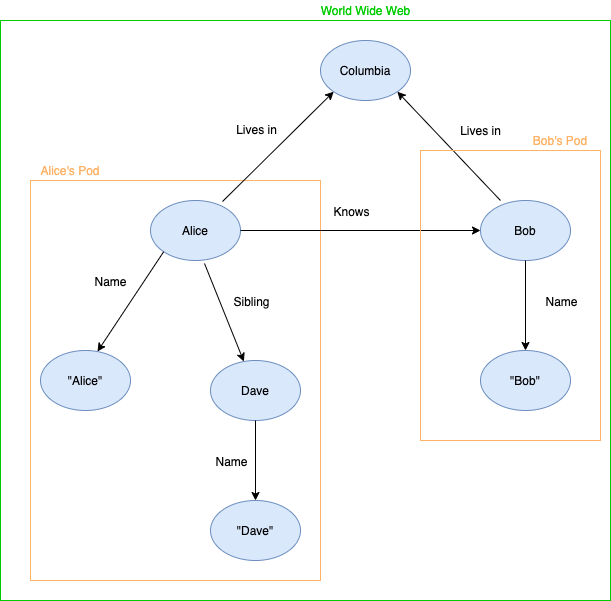
\includegraphics[width=\linewidth]{images/Linked Data Example.png}
    \caption{Linked Data voorbeeld}
    \label{fig:linked_data_example}
\end{figure}

Een voorbeeld van hoe het \textit{World Wide Web} eruit zou kunnen zien is geschetst in \figureref{fig:linked_data_example}. Dit voorbeeld toont de ideale situatie waar personen een eigen pod met informatie hebben. Zo hebben Alice en Bob elk hun eigen plaats op het web, waar informatie over hun te vinden is. Deze informatie zou onder andere hun naam, telefoonnummer, adres, interesses, werkomgeving, etc kunnen zijn. Daarnaast zijn er ook connecties tussen Alice en Bob. Om te beginnen is Bob gekend door Alice, waardoor er een verwijzing is naar meer context over Bob in zijn pod. Daarnaast wonen ze beide in dezelfde stad, waardoor het mogelijk is om bijvoorbeeld te zoeken naar iedereen die in een bepaalde stad woont. Al deze personen zullen terug te vinden zijn aan de hand van een verwijzing naar meer context (lees: meer informatie) over deze personen. Dit is echter een vereenvoudigd voorbeeld, in de reële situatie zijn er veel meer links en dit in alle richtingen.